\documentclass{article}
\usepackage[preprint, nonatbib]{nips_2018}
\usepackage{listings}
% to compile a preprint version, e.g., for submission to arXiv, add
% add the [preprint] option:
% \usepackage[preprint]{nips_2018}

% to compile a camera-ready version, add the [final] option, e.g.:
% \usepackage[final]{nips_2018}

% to avoid loading the natbib package, add option nonatbib:
% \usepackage[nonatbib]{nips_2018}

\usepackage{float}

\usepackage[square,numbers]{natbib}
\bibliographystyle{abbrvnat}

\usepackage[utf8]{inputenc} % allow utf-8 input
\usepackage[T1]{fontenc}    % use 8-bit T1 fonts
\usepackage{hyperref}       % hyperlinks
\usepackage{url}            % simple URL typesetting
\usepackage{booktabs}       % professional-quality tables
\usepackage{amsfonts}       % blackboard math symbols
\usepackage{nicefrac}       % compact symbols for 1/2, etc.
\usepackage{microtype}      % microtypography
\usepackage{graphicx}
\usepackage{tabularx}
\usepackage{hyperref}
\usepackage{amsmath}
\usepackage{gensymb}
\usepackage[polish]{babel}
\begin {document}
\title{
Sprawozdanie z zadania 3 \\
"Oświetlenie lokalne"}
\author{
Martyna Kochalska 331704,
Jakub Próchnicki  331730\\
}

\maketitle
\section{Cel projektu}
Projekt ma na celu zademonstrowanie techniki oświetlenia lokalnego z wykorzystaniem 
modelu Phonga i Phonga-Blina, a także uzyskanie chropowatości oświetlanych powierzchni
za pomocą techniki bump-mappingu.
\section{Program}
Program został napisany w języku Java wersja 21 w środowisku systemu Linux.
Wykorzystano biblioteki graficzne Swing oraz AWT.
\subsection{Prerekwizyty}
\begin{itemize}
    \item openjdk-21
    \item maven
\end{itemize}
\subsection{Instalacja i uruchomienie }
W celu skorzystania z programu należy np. w terminalu systemu Linux wykonać poniższe czynności.
Budowa projektu:
\begin{lstlisting}
mvn package
\end{lstlisting}
Uruchomienie:
\begin{lstlisting}
$ java -cp target/classes LocalLightingApp
\end{lstlisting}

\section{Scena}
W centum sceny znajduje się kula. Obraz kuli uzyskany jest w sposób przybliżony, 
tzn. wyświetlany jest okrąg, a cieniowanie modelu oświetlenia daje wrażenie głębi.
Promień okręgu ustawiony jest na 140 jednostek.Współrzędne sceny są zapisane
w układzie współrzędnych ekranu, gdzie początek przypada na lewy górny róg.
Lampa domyślnie położona jest 400 jenostek w prawo od lewej krawędzi ekranu,
200 jednostek w dół od górnej krawędzi i na tej samej głębokości. Kolor tła ustawiono na \#212121.

\section{Sterowanie żródłem światła}
W programie przewidziano możliwość zmiany pozycji źródła światła za pomocą następujących klawiszy:
\begin{itemize}
    \item Strzałka w górę - przesuwa źródło w górę względem kuli
    \item Strzałka w dół - przesuwa źródło w dół względem kuli 
    \item Strzałka w prawo - przesuwa źródło w prawo względem kuli 
    \item Strzałka w lewo - przesuwa źródło w lewo względem kuli  
\end{itemize}
Pojedyncza operacja zmienia daną współrzędną źródła o 20 jednostek.

\section{Model oświetlenia}
W programie zastosowano dwa warianty modelu Phonga w celu oświetlenia kuli.

\subsection{Klasyczny model Phonga}
\begin{center}
$I = I_a * k_a + I_p*k_d*f_{att}* (\vec{N} \cdot \vec{L}) + I_p * k_s* f_{att}* cos^{n}(\alpha)$, 
\end{center}
W naszym programie operujemy w 3 kanałach barw, co przyjmuje postać macierzową \\
\begin{center}
    $I=
    \begin{bmatrix}
        K_a^{(R)} & K_d^{(R)} &K_s^{(R)} \\
        K_a^{(G)} & K_d^{(G)} &K_s^{(G)} \\
        K_a^{(B)} & K_d^{(B)} &K_s^{(B)}\\
    \end{bmatrix}
    \begin{bmatrix}
        1 & 0 & 0 \\ 
        0 & (\vec{N} \cdot \vec{L}) & 0 \\ 
        0 & 0 & 1
    \end{bmatrix}
    \begin{bmatrix}
        1 & 0 & 0 \\ 
        0 & 1 & 0 \\
        0 & 0 & cos^n(\alpha)
    \end{bmatrix}
    \begin{bmatrix}
        1 & 0 \\
        0 & 1 \\ 
        0 & 1
    \end{bmatrix}
    \begin{bmatrix}
        1 & 0 \\
        0 & f_{att}
    \end{bmatrix}
    \begin{bmatrix}
        I_a \\ 
        I_p
    \end{bmatrix}$
\end{center}
gdzie:

$R,G,B$ - kanały barw \\
$I_a$ - natężenie światła z otoczenia \\
$k_a$ - współczynnik odbicia światła z otoczenia \\
$I_p$ - natęzenie światła punktowego \\
$k_d$ - współczynnik odbicia światła rozproszonego \\
$k_s$ - współczynnik odbicia światła kierunkowego \\
$f_{att}$ - współczynnik tłumienia źródła z odległością \\
$n$ - współczynnik gładkości powierzchni \\
$cos(a) = \vec{R} \cdot \vec{V}$ - kosinus kąta pomiędzy wektorem światła odbitego $\vec{R}$ a wektorem skierowanym do obserwatora $\vec{V}$

Wszystkie zdefiniowane tu paramtery mogą być w programie dostrajane przez użytkownika.
\subsection{Model Phonga-Blinna}
Jest to modyfikacja klasycznego modelu Phonga, która zmienia sposób liczenia wartości $cos(\alpha)$.

Wprowadzone jest pojęcie wektora połówkowego, zdefiniowanego w następujący sposób:

$\vec{H} = \frac{\vec{L}+\vec{V}}{||\vec{L}+\vec{V}||}$

\begin{figure}[H]
    \begin{center}
        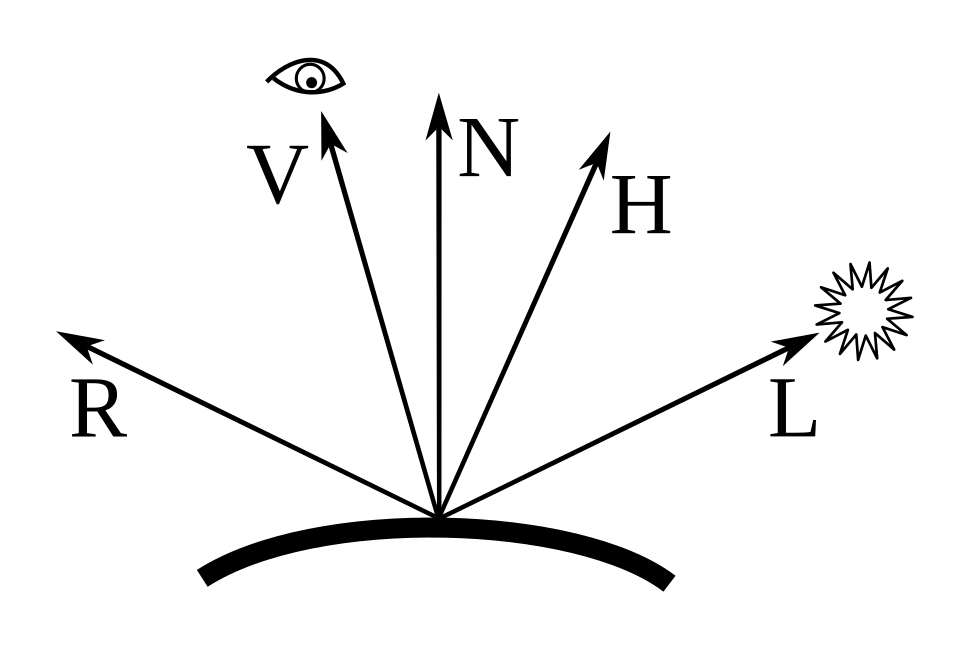
\includegraphics[width=0.5\linewidth]{img/Blinn_Vectors.png}
    \end{center}
    \caption{
        Układ wektorów w modelu Phonga-Blinna. Wektor H stanowi dwusieczną kąta pomiędzy
        normalną a wektorem do światła.
    }
\end{figure}
Wartość $cos(\alpha)$ liczona jest więc jako $\vec{N} * \vec{H}$, co w efekcie daje mniej
niż podejście w klasycznym modelu Phonga.

W programie w obu modelach znormalizowany wektor $\vec{V}$ skierowany do obserwatora wynosi [0,0,1], 
co jest równoznaczne z normalną do powierzchni kuli, prostopadłą do płaszczyzny równoległej
do ekranu. 

\section{Chropowatość powierzchni}
W celu modyfikacji faktury kuli zastosowano technikę bump-mappingu.
Wektor normalny w danym punkcie kuli został zmodyfikowany w następujący sposób:

\begin{center}
    $\vec{N'} = \vec{N} + F*\vec{N}$ , co definiujemy:

    $
    \begin{bmatrix}
        x_n \\ 
        y_n \\ 
        z_n
    \end{bmatrix}' =
    \begin{bmatrix}
        x_n \\ 
        y_n \\ 
        z_n
    \end{bmatrix}
    +
    b* sin(\begin{bmatrix}
        70 & 0 & 0\\ 
        0 & 98 & 0\\ 
        9.8 & 9.8 & 0
    \end{bmatrix}*
    \begin{bmatrix}
        x_n \\ 
        y_n \\ 
        z_n
    \end{bmatrix})
    $,
\end{center}
gdzie:\\

$b$ - to współczynnik zaburzenia, jest regulowany w menu programu.\\
Pozostałe współczynniki zostały dobrane eksperymentalnie

\section{Testy}
\subsection{Wygląd różnych materiałów}
\begin{figure}[H]
    \begin{center}
        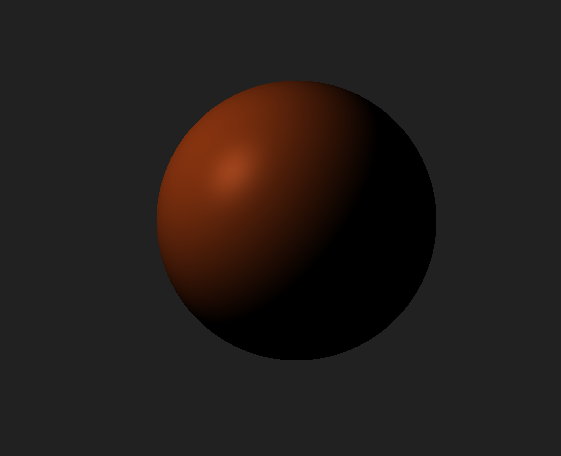
\includegraphics[width=0.7\linewidth]{img/copper.png}
    
    \caption{
        Uzyskana barwa miedzi, 
    } 
    
    
    \end{center}
\end{figure}
Powyższy obraz uzyskano dla następujących współczynników odbicia: 
\begin{center}
    $K=\begin{bmatrix}
        0.24725 & 0.75164 & 0.628281 \\
        0.1995 & 0.60648 & 0.555802 \\
        0.0745 & 0.22648 & 0.366065
    \end{bmatrix}$,
    $n = 12.8$
\end{center}


\begin{figure}[H]
    \begin{center}
        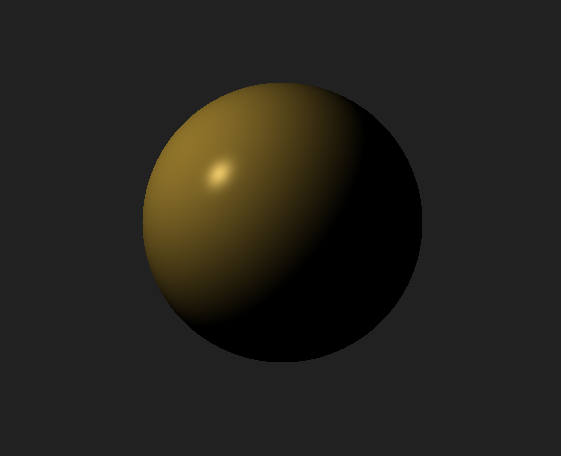
\includegraphics[width=0.7\linewidth]{img/gold.png}
    \end{center}
    \caption{
        Uzyskana barwa złota.
    }
\end{figure}
Powyższy obraz uzyskano dla następujących współczynników odbicia:
\begin{center}
$K=\begin{bmatrix}
    0.19125 & 0.7038 & 0.256777 \\
    0.0735 & 0.27048 & 0.137622 \\
    0.0225 & 0.0828 & 0.086014
\end{bmatrix}$,
$n = 51.2$
\end{center}

\begin{figure}[H]
    \begin{center}
        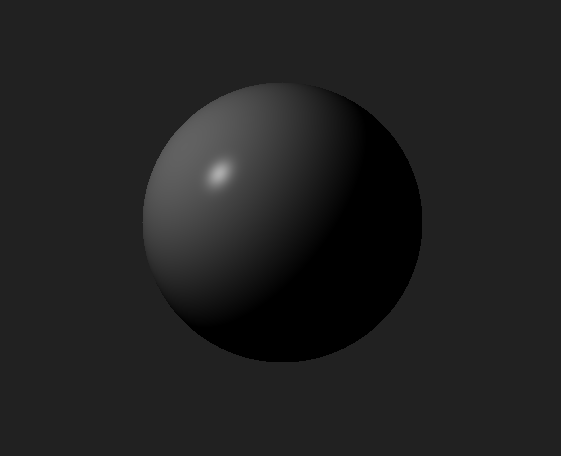
\includegraphics[width=0.7\linewidth]{img/silver.png}
    \end{center}
    \caption{
        Uzyskana barwa srebra.
    }
\end{figure}
Powyższy obraz uzyskano dla następujących współczynników odbicia:
\begin{center}
$K=\begin{bmatrix}
    0.19225 & 0.50754 & 0.508273 \\
    0.19225 & 0.50754 & 0.508273 \\
    0.19225 & 0.50754 & 0.508273
\end{bmatrix}$,
$n = 51.2$
\end{center}
\subsection{Manipulacja położeniem źródła światła}
\begin{figure}[H]
    \begin{center}
        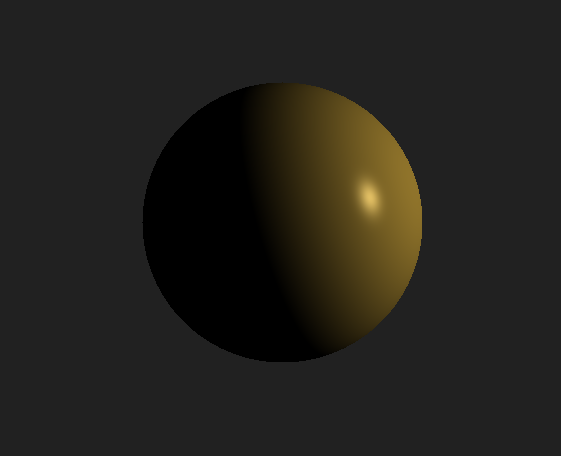
\includegraphics[width=0.7\linewidth]{img/lamp_right.png}
    \end{center}
    \caption{
        Przesunięcie źródła światła w prawo.
    }
\end{figure}
\begin{figure}[H]
    \begin{center}
        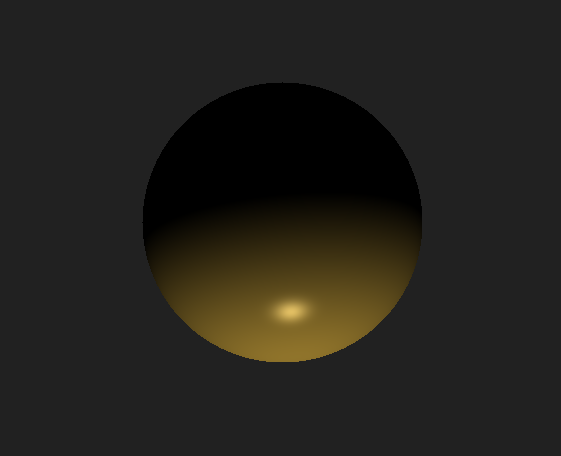
\includegraphics[width=0.7\linewidth]{img/lamp_down.png}
    \end{center}
    \caption{
        Przesunięcie źródła światła w dół.
    }
\end{figure}
\begin{figure}[H]
    \begin{center}
        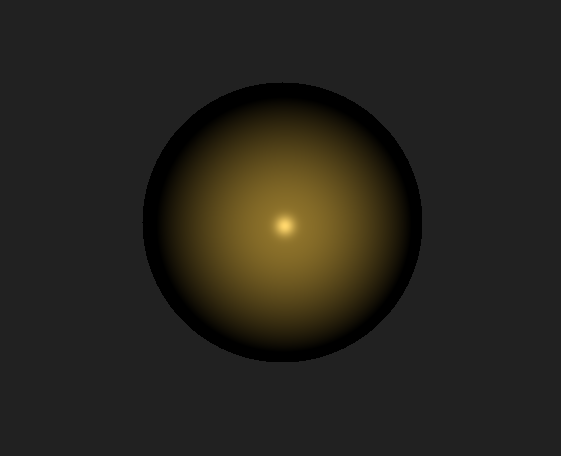
\includegraphics[width=0.7\linewidth]{img/lamp_center.png}
    \end{center}
    \caption{
        Przesunięcie źródła światła na środek.
    }
\end{figure}
\subsection{Manipulacja paramterami modelu}
\begin{figure}[H]
    \begin{center}
        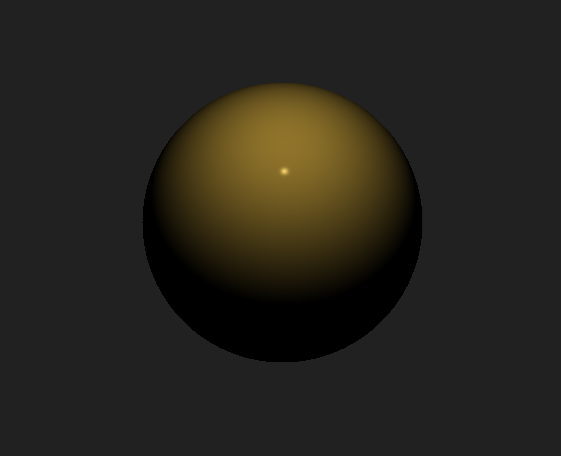
\includegraphics[width=0.7\linewidth]{img/big_n.png}
    \end{center}
    \caption{
        Dziesięciokrotne zwiększenie wykładnika
        względem stanu prezentowanego w poprzedniej sekcji.
        Plamka znacząco się zmniejszyła, co jest właściwą odpowiedzią modelu.
    }
\end{figure}

\begin{figure}[H]
    \begin{center}
        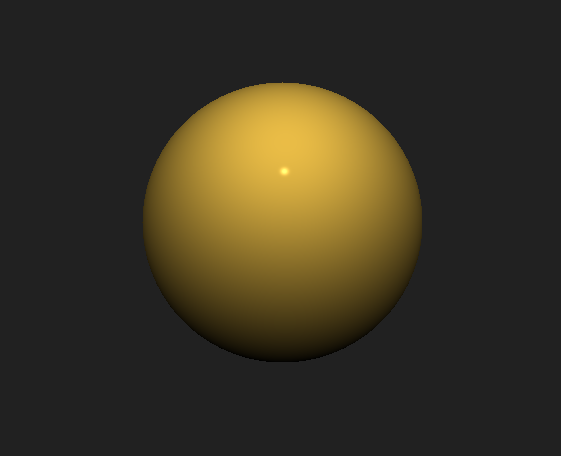
\includegraphics[width=0.7\linewidth]{img/greater_ambient_intesity.png}
    \end{center}
    \caption{
        Znaczące zwiększenie intensywności światła z otoczenia.
        Obszary zacienione mocno się zredukowały, co również
        jest poprawną reakcją modelu.
    }
\end{figure}

\begin{figure}[H]
    \begin{center}
        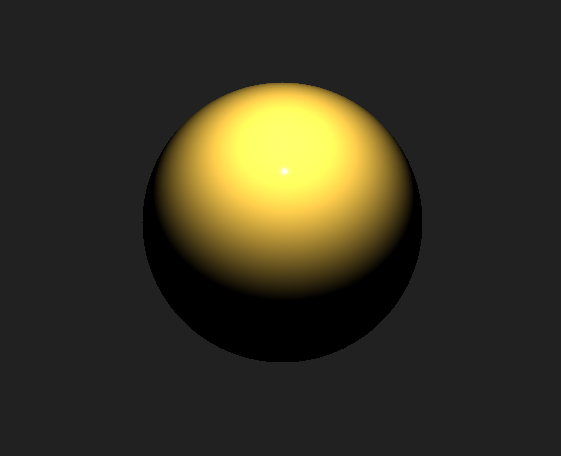
\includegraphics[width=0.7\linewidth]{img/greater_point_intesity.png}
    \end{center}
    \caption{
        Znaczące zwiększenie intensywności światła punktowego.
        Obserwuje się mocne rozjaśnienie obszarów w okolicy punktu 
        padania światła na powierzchnię kuli przy jednoczesnym niewielkim
        naruszeniu obszarów zacienionych. Jest to poprawna odpowiedź modelu.
    }
\end{figure}

\begin{figure}[H]
    \begin{center}
        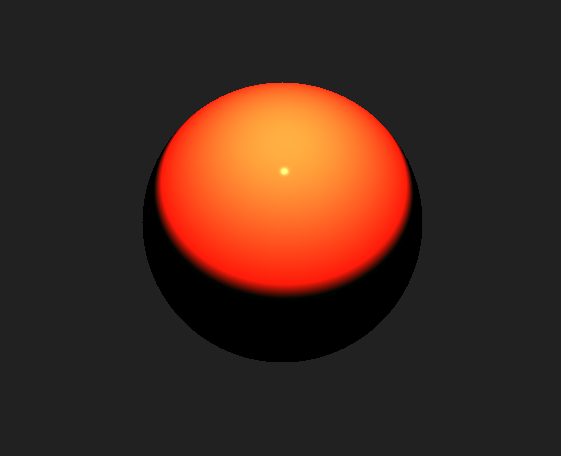
\includegraphics[width=0.7\linewidth]{img/greater_R_diffuse_reflection.png}
    \end{center}
    \caption{
        Znaczące zwiększenie współczynnika odbicia światła rozproszonego w kanale
        czerwonym powoduje degenerację barwy i zwiększenie udziału koloru czerwonego 
        przy jednoczesnym większym zmatowieniu powierzchni, co jest właśiwą reakcją
        modelu.
    }
\end{figure}

\subsection{Porównanie obu modeli}

\begin{figure}[H]
    \begin{center}
        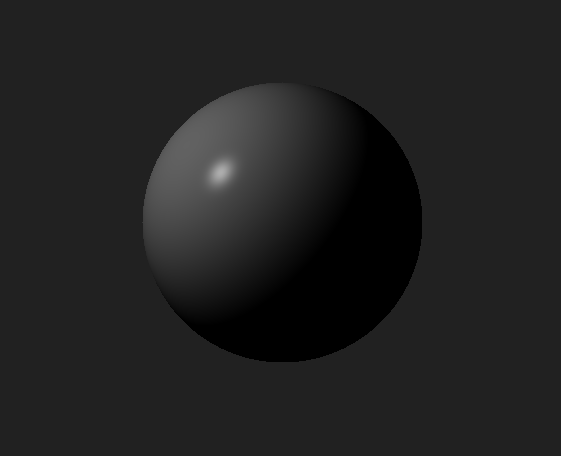
\includegraphics[width=0.7\linewidth]{img/classical_phong.png}
    \end{center}
    \caption{
        Widok kuli srebra w klasycznym modelu Phonga.
    }
\end{figure}

\begin{figure}[H]
    \begin{center}
        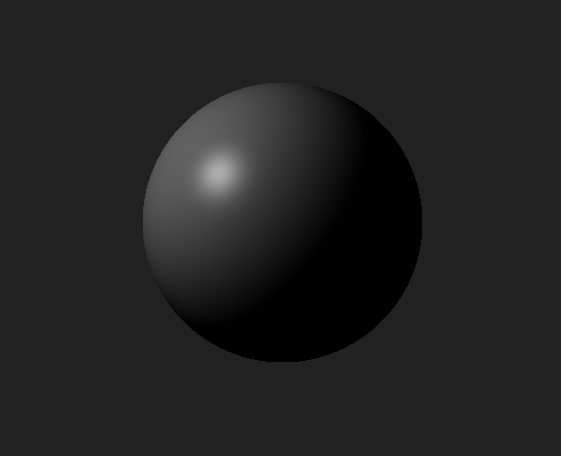
\includegraphics[width=0.7\linewidth]{img/phong-blinn.png}
    \end{center}
    \caption{
        Widok tej damej kuli przy identycznych parametrach w modelu Phonga-Blinna.
        Widać większe rozmycie plamki, wynikające z mniejszej wartości kosinusa kąta w obliczeniach
        światła kierunkowego.
    }
\end{figure}
\subsection{Manipulacja fakturą materiału}

\begin{figure}[H]
    \begin{center}
        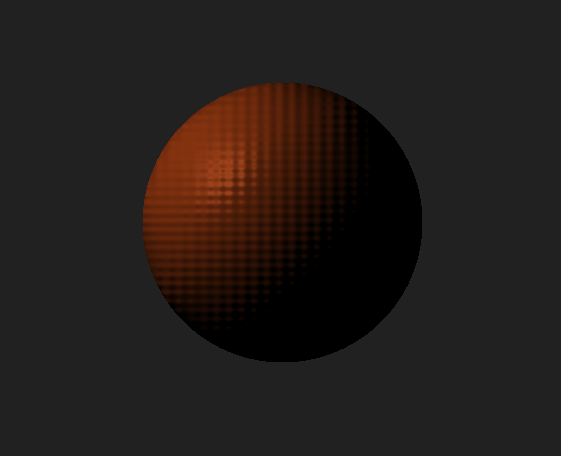
\includegraphics[width=0.7\linewidth]{img/bump_mapping1.png}
    \end{center}
    \caption{
        Widok kuli miedzi w modelu Phonga dla współczynnika b 
        zdefiniowanego w tym sprawozdaniu równego 0.1
    }
\end{figure}

\begin{figure}[H]
    \begin{center}
        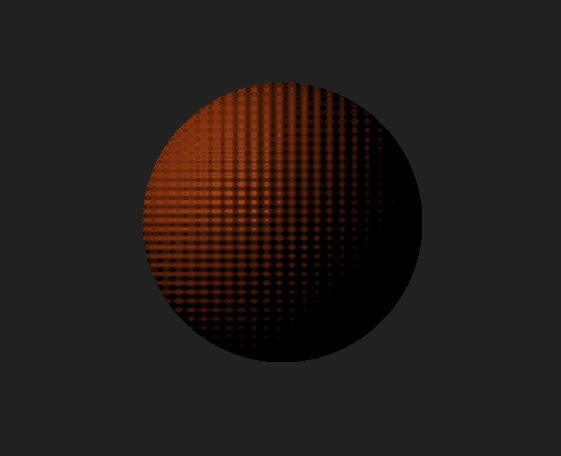
\includegraphics[width=0.7\linewidth]{img/bump_mapping2.png}
    \end{center}
    \caption{
        Widok kuli miedzi w modelu Phonga dla współczynnika b równego 0.3
    }
\end{figure}

\end{document}
